\documentclass[../PhD.tex]{subfiles}

\begin{document}

%%%%%%%%%%%%%%%%%%%%%%%%%%%%%%%%%%%%%%%%%%%%%%%%%%%%%%
%%%%%%%%%%%%%%%%%%%%%%%%%%%%%%%%%%%%%%%%%%%%%%%%%%%%%%

\chapter{Introduction}
\label{ch: intro}

As experimental research into quantum information, condensed matter, and nuclear physics continues to reach new levels of precision, progress in developing theoretical predictions in these fields is hindered by a fundamental problem: in strong coupling regimes, the perturbative methods that underpin theories such as Quantum Electrodynamics become invalid. This is because such systems are highly nonlinear. While some progress is possible by employing numerical schemes such as lattice approximations, analytical results remain beyond our current mathematical understanding. In order to make progress, a new paradigm was required. By considering different coupling limits of a single string theory, \cite{hep-th/9711200} established a holographic description between strongly-coupled gauge theories and weakly-coupled gravitational theories in one higher dimension. Since its inception, this duality has been further developed into a dictionary that relates the fields in the gravitational theory to operators in the gauge theory. The Anti-de Sitter/Conformal Field Theory (AdS/CFT) correspondence allows strongly-coupled quantum processes to be reliably examined via geometric quantities in the dual theory. This duality has become a standard tool for theoretical physicists studying all kinds of dynamic processes in quantum theories, including the out-of-equilibrium dynamics of quantum theories at strong coupling.

The goal of this thesis is to leverage the AdS/CFT correspondence to study the dynamics of strongly coupled quantum theories through their dual description as a weakly coupled gravitational theory. To do so, we focus on minimally coupled scalar fields in Einstein-Hilbert gravity on AdS backgrounds. Existing entries in the gauge/gravity dictionary will motivate the systems that are considered, and existing literature will point to areas within the topic that have yet to be explored. The nonlinear stability of the theory will be studied via both numerical and analytical methods. We will see that gravitational collapse in the bulk theory signals a phase transition in the dual gauge theory, and so examining the dynamics of the collapse is tantamount to understanding time dependent processes in the boundary theory.

This thesis contains three manuscripts that either have been, or are about to be, submitted for publication. In chapter~\ref{ch: massive}, we examine the limits of the nonlinear stability of AdS$_5$ by examining the range of behaviours exhibited by differing initial data with static boundary conditions. Next, in chapter~\ref{ch: ttf}, we expand upon solutions to the perturbative theory that capture the weakly turbulent dynamics involved in the collapse process. We focus on determining the stability of solutions to the leading nonlinear contributions to the perturbative theory, known as quasi-periodic solutions. We then evolve these solutions in the perturbative framework and evaluate their longevity beyond the perturbative time scale. Finally, in chapter~\ref{ch: driven} we consider the addition of a time-dependent source term on the conformal boundary of the gravitational theory and derive the renormalization flow equations for the first non-trivial order in the small-amplitude expansion. A discussion of the results follows in chapter~\ref{ch: conclusion}.

However, before utilizing the correspondence to study any particular process, we first review the main tenet of the gauge/gravity duality and its consequences: that there exists a fundamental relationship between a conformal field theory in $d$-dimensions and a gravitational theory in ($d + 1$)-dimensions.

%%%%%%%%%%%%%%%%%%%%%%%%%%%%%%%%%%%%%%%%%%%%%%%%%%%%%%%
%%%%%%%%%%%%%%%%%%%%%%%%%%%%%%%%%%%%%%%%%%%%%%%%%%%%%%%

\section{The AdS/CFT Correspondence}
\label{sec: ads/cft}

It was shown by \cite{hep-th/9711200} that a non-perturbative correspondence existed between superconformal field theories and supergravity theories on various spacetimes. Although originally conjectured from the perspective of string theory, more modern reviews of the gauge/gravity duality establish a gravitational theory as arising from the strong coupling limit of a gauge theory; see \cite{gr-qc/0602037} for a review. We will use this paradigm to heuristically motivate the duality, as well as introduce relevant relationships between quantities in either theory.  

%%%%%%%%%%%%%%%%%%%%%%%%%%%%%%%%%%%%%%%%%%%%%%%%%%%%%%%

\subsection{Extra Dimensions In Gauge Theories}
\label{ssec: extra dims in gauge theories}

Although \cite{hep-th/9711200} was the first to establish explicitly a correspondence between a gravitational theory in $(d+1)$-dimensional AdS and a conformal field theory in $d$-dimensions, the concept of a holographic relationship between a gauge theory and a gravitational theory in one higher dimension was conjectured earlier by \cite{gr-qc/9310026} and \cite{hep-th/9409089} without relying solely on string theory. 

For most gauge theories, there is a running of the coupling that dictates the evolution of the couplings with energy. Therefore, the physics of the theory is local with respect to an extra dimension, the energy. However, since many gauge theories suffer UV divergences at large energies, the size of the extra dimension may be limited. In contrast, supersymmetric theories have vanishing beta functions; therefore, there is no running of the coupling. In this case, the energy scale is arbitrary and the extra dimension of the theory has no bound.

The vanishing of the beta function also indicates that the conformal invariance of the theory is unbroken; conformal invariance requires (among other things) that the theory remain invariant under rigid scale transformations by a unitless constant $a$, such that $x^\mu \to a x^\mu$. Interpreting the energy scale as an extra dimension, $r$, we require it to transform in the same way as energy, so that $r \to r/ a$. The most generic metric that also obeys Poincar\'e plus scale symmetries is
\begin{align}
\label{Poincare ads}
ds^2 = \frac{a^2}{z^2} \left( \eta_{\mu \nu}dx^\mu dx^\nu +dz^2 \right) \, ,
\end{align}
where $z = a^2 / r$. This is precisely the metric for Anti-de Sitter space with characteristic length $a$. 

More than being an \emph{a posteriori} observation, the gauge/gravity correspondence is in fact a much deeper and more specific relationship. The derivation of the duality is thoroughly covered from the full string theory perspective in, among others, \cite{hep-th/9711200, gr-qc/0602037, hep-th/9902131, hep-th/9905111}. For now, let us establish the duality that will be most applicable to us: the duality between type IIb supergravity on conformal \ads and $\mc N = 4$ supersymmetric Yang-Mills theory in $(3+1)$-dimensions.

%%%%%%%%%%%%%%%%%%%%%%%%%%%%%%%%%%%%%%%%%%%%%%%%%%%%%%%

\subsection{The AdS$_5 \times$S$^5$ Duality}
\label{ssec: AdS5xS5}

Consider a stack of $N$ coincident D3-branes in type IIb string theory (ten Minkowski dimensions), each of which couple to gravity with strength $g_s$. At weak coupling, $g_s N \ll 1$, there are closed string states as well as open strings that end on the branes and have an $SU(N)$ super-Yang-Mills effective action. At strong coupling, however, the branes curve the background and source an extremal black-brane geometry \cite{Zwiebach:2004tj}, whose metric is
\begin{align}
\label{bb geom}
ds^2 = f(r)^{-1/2} \eta_{\mu \nu} dx^\mu dx^\nu + f(r)^{1/2} \left(  dr^2 + r^2 d\Omega_5^2 \right)  \quad  \text{with} \quad f(r) = 1 + \frac{4 \pi g_s N \ell_s^4}{r^4} \, ,
\end{align}
where the $x^\mu$ span the worldvolume of the D3-branes, $d\Omega_5^2$ is the metric of the unit 5-sphere, and $\ell_s$ is the length of the string.

Now we take the low-energy limit of the theories at either coupling limit. At weak coupling, the open strings decouple from the closed strings, resulting in an $SU(N)$ super-Yang-Mills gauge theory on the brane worldvolume. In the $g_s N \gg 1$ case, the low-energy limit corresponds to the near-horizon limit, $r \to 0$. In this limit, the 10D metric factors into the product AdS$_5 \times$S$^5$. To see this, we define $\ell \equiv (4\pi g_s N)^{1/4} \ell_s$, so that $f^{1/2}(r) \to \ell^2 / r^2$ in the near-horizon limit and \eqref{bb geom} becomes
\begin{align}
\label{param rels}
ds^2 = \frac{r^2}{\ell^2} \eta_{\mu \nu} dx^\mu dx^\nu + \frac{\ell^2}{r^2}dr^2 + \ell^2 d\Omega_5^2 \, .
\end{align}
Note that the branes are now located at the bottom of the infinite throat. Any states near the horizon will be redshifted to low energies and any states in the asymptotic region will decouple from states near the black branes; all that remains are closed string states, i.e.~supergravity, on an asymptotically AdS$_5$ background. This motivates the duality we will examine in detail: the one between scalar fields in \ads and a supersymmetric $SU(N)$ Yang-Mills gauge theory on the boundary of AdS$_5$.

Given that we now know what string theory we are working with, we can more directly relate the dimensionless parameters of the string theory (i.e.~the string coupling $g_s$ and AdS scale in string units, $\ell / \ell_s$) to the dimensionless parameters of the CFT (i.e.~the Yang-Mills coupling $g_{YM}$ and colour number $N$). By examining the D3-brane Lagrangian, we are able to relate $g_{YM}$ and $g_s$ through $4\pi g_s = g_{YM}^2$. Altogether,
\begin{align}
\label{params}
4\pi g_s = g_{YM}^2 \sim \frac{\lambda}{N} \quad \text{and} \quad \frac{\ell}{\ell_s} = \left( 4\pi g_s N \right)^{1/4} \sim \lambda^{1/4} \, ,
\end{align}
where $\lambda$ is the 't Hooft coupling $\lambda \equiv g_s N = g_{YM}^2 N$. To remove stringy corrections to the geometry, $\ell / \ell_s \gg 1$ so that the AdS length is much larger than the string length. Furthermore, string interactions are suppressed when $g_s \ll 1$. Thus, the bulk theory approaches  classical Einstein-Hilbert gravity when $N \gg \lambda \gg 1$.

By considering other superstring avatars, such as M-theory\footnote{M-theory is the strong-coupling limit of type IIa superstring theory on 11D spacetime, and can be mapped to the other 10D superstring theories through choices of compactifications and length/coupling dualities \cite{Polchinski:1998rr}.}, we are able to establish similar dualities between gravitational and conformal field theories. In particular, the M-theory equivalent of D$2$-branes, M$2$-branes, are used -- along with corresponding coupling limits -- to establish a duality between a gravitational bulk theory on AdS$_4 \times$S$^7$ and a CFT in $(2+1)$-dimensions \cite{hep-th/9711200}. In fact, many such dualities can be constructed through applying different compactifications and/or sources in the extra dimensions, each of which describes a different type of CFT on the boundary. For a review of other types of holographic constructions, see e.g.~\cite{1612.07324, 1501.00007}.

\vspace{-0.2in}

%%%%%%%%%%%%%%%%%%%%%%%%%%%%%%%%%%%%%%%%%%%%%%%%%%%%%%%
%%%%%%%%%%%%%%%%%%%%%%%%%%%%%%%%%%%%%%%%%%%%%%%%%%%%%%%

\section{The Gauge/Gravity Dictionary}
\label{ssec: dictionary}

\vspace{-0.1in}

With the existence of the duality now motivated, we turn to what kind of predictions arise from the correspondence. In particular, we wish to establish what physical quantities in either theory can be related through the AdS/CFT correspondence. In fact, many such relations arose from efforts to find counterexamples to the correspondence in the hopes of disproving it. Instead, each attempt confirmed the AdS/CFT correspondence and became an entry in the so-called dictionary. Here we will provide a few example cases to motivate how quantities on either side of the correspondence can be related.

{\bf Symmetries}

Consider the symmetries present in the \ads bulk theory. A $(p+2)$-dimensional Anti-de Sitter space can be presented by the hyperboloid $X_0^2 + X^2_{p+2} - \sum^{p+1}_{i=1} X_i^2 = R^2$ in a $(p+3)$-dimensional space with the metric
\begin{align}
\label{ads hyperboloid}
ds^2 = -dX_0^2 - dX_{p+2}^2 + \sum^{p+1}_{i = 1} dX^2_i \, .
\end{align}
The choice of {$X_0 = R \cosh \rho \, \cos \tau$}, {$X_{p+2} = R\cosh \rho \,\sin \tau$}, and {$X_i = R \sinh \rho \,\Omega_i$} with $i=1,\ldots,p + 1$, $0 \leq \rho$, $0 \leq \tau \leq 2\pi$, and $\sum_i \Omega_i = 1$ covers the hyperboloid exactly once, and is known as global coordinates. In these coordinates, the metric on AdS$_{p+2}$ is
\begin{align}
\label{global ads 1}
ds^2 = R^2 \left( - \cosh^2 \rho~d\tau^2 + d \rho^2 + \sinh^2 \rho~d\Omega^2 \right) \, .
\end{align}
A common coordinate redefinition of $\tan x = \sinh \rho$ maps spatial infinity to $x = \pi / 2$, and allows \eqref{global ads 1} to be written as
\begin{align}
\label{global ads 2}
ds^2 = \frac{R^2}{\cos^2 x} \left( - d\tau^2 + dx^2 + \sin^2 x~d\Omega^2 \right) \, .
\end{align}
Another common parameterization of AdS is a set of coordinates that cover half of the hyperboloid \eqref{ads hyperboloid}, known as Poincar\'e coordinates. These set {$X_0 = (1 + z^2 (R^2 + {\vec x}^2 - t^2) )/2z$}, {$X_{p+2} = Rz t$}, {$X^{p+1} = ( 1 - z^2 (R^2 - {\vec x}^2 + t^2) )/ 2z$}, and {$X^i = Rzx^i$}, with {$i = 1, \ldots, p$}, {$z > 0$}, and {$\vec x \in \mathbb{R}^p$}. Thus, the metric of AdS$_{p+2}$ in the Poincar\'e patch description is
\begin{align}
\label{poincare ads}
ds^2 = R^2 \left( \frac{d^2z}{z^2} + z^2 (- dt^2 + d {\vec x}^2) \right) \, .
\end{align}

AdS$_{p+2}$ has the isometry $SO(2,p+1)$, and is homogeneous and isotropic \cite{hep-th/9905111}. The global coordinate representation helps us to interpret the maximal compact subgroup of $SO(2, p+1)$, $SO(2)\times SO(p+1)$, as constant translations in $\tau$ plus rotations of S$^p$. Likewise, the Poincar\'e coordinates describe the symmetries of AdS in terms of the Poincar\'e transformation on $(t, \vec x)$ plus the dilatation transformation {$(t, \vec x, z) \to (ct, c \vec x, c^{-1}z)$} for $z >0$. Finally, invariance under special conformal transformations makes the Poincar\'e patch description of AdS fully invariant under conformal coordinate transformations.

In particular, a bulk theory on \ads has $SO(2,4)\times SO(6)$ symmetry. The gauge theory on the boundary of this space has an $SO(2,4)$ isometry from its conformal invariance, as well as $SU(4) \simeq SO(6)$ R-symmetry that relates the six scalar fields and four fermions of the theory \cite{hep-th/9711200}. Therefore, the spatial isometries of the bulk space are interpreted as global symmetries of the boundary theory. Additionally, the supersymmetries inherent in the original type IIb superstring theory remain unbroken by the strong/weak coupling limits. Hence, the gauge/gravity correspondence conserves the symmetries of both theories.

{\bf Observables}

Besides matching symmetry groups and relating dimensionless parameters, the AdS/CFT correspondence is able to produce more physically relevant relationships involving observables in either theory. One such concrete example comes from relating the asymptotic behaviour of bulk fields to the expectation values of operators in the boundary theory: a bulk field in Poincar\'e AdS with metric \eqref{Poincare ads} has leading-order value $\phi^{(0)}$ as $z \to 0$ (i.e.~as the conformal boundary is approached) and acts as a source for an operator $\mc O$ on the boundary. Furthermore, by examining the next-to-leading order contribution to the bulk field, $\phi^{(1)}$, it can be shown that the expectation value of the operator is given by $\langle \mc O \rangle \propto \phi^{(1)}$ \cite{hep-th/9905104}. In \S~\!\ref{ssec: scalar fields}, we use the gauge/gravity duality to calculate the mass dimension of the boundary operator $\mc O$.

Another such example is the quark anti-quark potential in the boundary theory. In the gauge theory, this can be calculated via the Wilson loop $W(\mathcal C)$, where $\mathcal C$ is the closed loop connecting the quark worldlines. The bulk interpretation of the Wilson loop is the extremized proper area of a string worldsheet anchored on $\mathcal C$ and extending into $z > 0$ \cite{hep-th/9803002}. 

\pagebreak

{\bf Entanglement Entropy}

A significant utilization of the gauge/gravity duality comes from its unique ability to relate quantum characteristics of the gauge theory to geometric ones in the bulk. Among the most quantum of all characteristics is the spatial distribution of quantum correlations within a system, given by the entanglement entropy. For a given subsystem $\mc M$ of a local field theory with reduced density matrix $\rho_{\mc M}$, the entanglement entropy is given by the Von Neumann entropy $S_{\mc M} = - \text{Tr} \rho_{\mc M} \ln \rho_{\mc M}$. In practice, $\mc M$ is a spatial region that is bounded by the entangling surface $\p \mc M$.

In the strong coupling limit, calculating the entanglement entropy can be prohibitively difficult. However, using the AdS/CFT correspondence it has been shown that $S_{\mc M}$ is given by a quarter of the area of the minimal surface at constant time in the bulk that is anchored on $\p \mc M$ \cite{hep-th/0603001}. Further properties of the entanglement entropy were subsequently shown to also have dual geometric descriptions in the bulk \cite{1304.4926}.

{\bf Partition Functions}

Since the underpinning of the AdS/CFT correspondence is taking different limits of the same theory, it is natural that the partition functions of either limit must still agree. We have already seen in \S~\!\ref{ssec: AdS5xS5} that the weak coupling limit of the type IIb string theory is supergravity (SUGRA) in the bulk, while the strong coupling limit gives a supersymmetric (SUSY) Yang-Mills gauge theory on the boundary. The gauge/gravity duality allows us to relate the two limits of the partition function:
\begin{align}
\label{partition functions}
e^{-S_{SUGRA}} \approx Z_{string} \simeq Z_{gauge} = e^{-W_{SUSY}} \, ,
\end{align}
where $W$ is the generating functional for connected Green's functions in the gauge theory.

Consider a massive bulk field $\phi(\vec x,z)$ that takes the value $\phi(\vec x, z=0) = \phi_0 (\vec x)$ on the conformal boundary. We then solve the bulk equations of motion away from the boundary (i.e.~$z > \epsilon$) subject to Dirichlet boundary conditions. The leading term in the epsilon expansion of the bulk field is $\phi(\vec x, z=\epsilon) \sim \epsilon^{\Delta^\pm} \phi_0(\vec x)$, where the scaling dimension $\Delta^\pm$ will be explicitly derived below. By definition, $S_{SUGRA}$ is extremized by this solution and so \eqref{partition functions} becomes \cite{hep-th/9802109, hep-th/9802150}
\begin{align}
\label{ads/cft duality}
\lim_{\epsilon \to 0} \big( S_{SUGRA} \left[ \phi(\vec x, z) \right] \big) \Big|_{\phi (\vec x, \epsilon) \to \phi_0(\vec x)} \simeq \left\langle \int d^dx \, \phi_0(\vec x) \mc O(\vec x) \right\rangle_{CFT} \, .
\end{align}

We will see that bulk scalar fields play an important role in the dual description of the thermalization of a CFT, as well as being a useful tool to study the nonlinear stability of AdS itself. 

{\bf Black Holes}

Another important ingredient of the AdS/CFT correspondence was first mentioned in \S~\!\ref{ssec: AdS5xS5}: black holes. As discussed previously, the weak coupling limit of the $N$ D3-branes produced an extremal black-brane geometry given by \eqref{param rels}, which is the Poincar\'e patch description of AdS. Since the interaction cross-section of the branes with low-energy states in the bulk shrinks to zero, the effective geometry for these states is Anti-de Sitter. When discussing black holes in the AdS/CFT correspondence, we are referring to black holes embedded within an AdS geometry. 

The connection between black hole physics and thermodynamics was noted by \cite{Bekenstein:1973ur}, and has been thoroughly examined since then. For a review of the thermodynamic properties of black holes, see \cite{Jacobson1996, Bardeen:1973gs, 1803.03633}. It suffices for our purposes to highlight a few key features of the thermodynamic properties of black holes, and thereby motivate a correspondence between black holes in the bulk theory and a gauge theory in thermal equilibrium on the boundary.

By considering quantum effects near the event horizon, it can be shown that black holes emit particles whose thermal spectrum is equivalent to a black body of temperature \cite{Hawking:1974rv, Hawking:1974sw}
\begin{align}
\label{hawking temp}
T_H = \frac{(\ell^2 + 2r_H^2)}{2 \pi r_H \ell^2} \, ,
\end{align}
where $r_H$ is the size of the event horizon. When the black hole is placed in a geometry with a conformal boundary, it will be in thermal equilibrium with its Hawking radiation, and a stationary observer at asymptotic infinity will observe a black body spectrum corresponding to the temperature $T_H$ \cite{Carroll:2004st}. The black hole will have positive specific heat, and therefore be thermodynamically stable, for $\ell \gg r_H$ so that $T_H \simeq 1/2\pi r_H$ \cite{Hawking:1982dh}. 

Now consider the partition function for a thermal system in contact with a heat reservoir at temperature $\beta^{-1}$. The quantum partition function involves the trace over the eigenvectors of the Hamiltonian,
\begin{align}
\label{quantum par}
Z = \text{Tr} \, e^{- \beta H} = \int dq \, \langle q | \exp ( - \beta H ) | q \rangle \, .
\end{align}
The trace vanishes by orthogonality of states except when the states have periodicity such that $q(0) = q(\beta)$. It then reduces to a sum over over only the periodic states \cite{Schellekens}
\begin{align}
\label{cft trace}
\text{Tr} \, e^{ - \beta H} = \int dq \int^{q'(\beta)=q}_{q'(0)=q} [dq'] \, e^{-S_E[q']} = \int [dq]_P \, e^{-S_E[q]} \, ,
\end{align}
where $S_E$ is the Euclidean action. Equivalently, we may sum over all states but impose the periodicity condition $\tau \sim \tau + \beta$. 

Now, we place this quantum theory in the background of a Schwarzschild black hole. After Wick rotating $t \to i\tau$, the metric is
\begin{align}
\label{Euclidean}
ds^2 = +\left(1 - \frac{2GM}{r} \right) d\tau^2 + \left(1 - \frac{2GM}{r}\right)^{-1}dr^2 + r^2 d\Omega_{d-1}^2 \, .
\end{align}
Note that within the horizon $r < 2GM$, the metric of \eqref{Euclidean} is no longer Euclidean but instead is $\text{diag}(- - + +)$, unlike the Lorentz signature metric where the time and radial position change roles without changing the signature. Taking the near-horizon limit, we see that the metric develops a conical singularity. To resolve the singularity at $r=r_H$, we require that the Euclidean time be periodic such that $\tau \sim \tau + 2\pi r_H$ \cite{hep-th/9803131}. By matching this condition on $\tau$ with the one from finite-temperature quantum system, we can see that 
\begin{align}
\label{temp/grav}
\left. \begin{aligned}
	\text{black hole:} &\quad \tau \sim \tau + 2\pi r_H \\
	\text{CFT:} &\quad \tau \sim \tau + \beta
	\end{aligned}
\: \right\} \: \beta \sim 2\pi r_H \quad \Rightarrow \quad T \sim 1/ 2\pi r_H \, .
\end{align}
Therefore, the temperature of the thermalized CFT is equal to the Hawking temperature of the black hole.

A non-trivial check of this duality comes from a comparison of the entropies of the two systems. In the bulk, the Bekenstein-Hawking relationship relates the entropy of a 5D black hole to the surface area of the horizon \cite{Bekenstein:1973ur}
\begin{align}
\label{bh dual entropy}
S_{BH} = \frac{A}{4G^{(5)}} \sim \frac{r_+^3 \ell^5}{g_s^2 \ell_s^8} \sim \frac{T_H^3 \ell^{11}}{g_s^2 \ell_s^8} \sim N^2 T_H^3 \ell^3 \, ,
\end{align}
where we have used the fact that the gravitational constant scales with dimension as $G^{(d)} \sim g_s^2 \ell_s^{d-2}$ as well as \eqref{params}. On the other hand, the entropy of a 4D gauge theory with temperature $T_H$ in the limit of weak coupling\footnote{In the strong coupling limit, the Yang-Mills degrees of freedom are interacting and the entropy calculation is not straightforward. However, the weak coupling limit can be smoothly interpolated to the strong coupling limit via a numerical factor that does not affect our comparison \cite{gr-qc/0602037}.} is
\begin{align}
\label{gauge dual entropy}
S_{YM} \sim N^2 T_H^3 \ell^3 \, .
\end{align}
This agreement shows that the gauge theory possesses enough states to match the entropy of black holes in AdS$_5$.

%%%%%%%%%%%%%%%%%%%%%%%%%%%%%%%%%%%%%%%%%%%%%%%%%%%%%%%
%%%%%%%%%%%%%%%%%%%%%%%%%%%%%%%%%%%%%%%%%%%%%%%%%%%%%%%

\section{Gravitational Collapse of Scalar Fields}
\label{sec: grav collapse}

The picture thus far is this: using the AdS/CFT correspondence, we are able to study strongly-coupled gauge theories through their holographic dual, which is a gravitational theory in Anti-de Sitter space with a conformal boundary. We have also seen that black hole solutions in the bulk correspond to thermal states in the boundary theory, and were able to derive the equilibrium temperature of the thermal system by examining the Hawking temperature of the black hole. These results are concern stationary systems; indeed, equilibrium and near-equilibrium dynamics of thermal gauge theories have holographic descriptions that are already understood (see \cite{1101.0618}, etc. for reviews). But what about the dynamics of the thermalization? 

Consider some gauge theory that is subjected to a homogeneous injection of energy on a very short time scale such that it is instantaneously far from equilibrium. The subsequent evolution towards a new equilibrium state is known as a \emph{quench}. Quenches can result in thermal states, meta-stable configurations, or may never equilibrate \cite{1103.2683}. For example, the infall of a spherical shell of matter (scalar field) in AdS is used as a model for the quench of a coherent state in a confined gauge theory. The radial position of the shell in the bulk acts as a scale to measure the typical separation of entangled excitations \cite{0705.0016}. As the shell falls towards the origin, one of two things can happen: if the shell has a high enough mass density, a black hole forms which signals the thermalization of the gauge theory; if the shell does not collapse, it can scatter off itself and begin expanding. Once the shell reaches the AdS boundary, the matter is reflected (under appropriate boundary conditions) and begins the infall again. This cycle of bounces is the holographic dual of so-called \emph{revivals} in the quantum theory \cite{1410.6201, 1412.6002}, and has been used to help explain results from cold atom experiments \cite{Dziarmaga2010, 2011arXiv1106.3567L}. The negative curvature of AdS allows for states that do not immediately thermalize to oscillate around the minimum of an effective potential, undergoing repeated gravitational focusing with each oscillation. Therefore, unlike in asymptotically flat space, thermalization can occur at long times with respect to the light crossing time. One may also wish to investigate other non-equilibrium processes, for example the spontaneous breaking of a discrete symmetry in the boundary CFT. The holographic dual description is the evolution from a bulk black hole to a hairy black hole \cite{1704.05454, 1902.08669}. However, the focus of the work in this thesis will be to study the dynamics of thermalization from a coherent state via the collapse of a scalar field.

%%%%%%%%%%%%%%%%%%%%%%%%%%%%%%%%%%%%%%%%%%%%%%%%%%%%%%%

\subsection{Scalar Fields in Holographic AdS$_{d+1}$}
\label{ssec: scalar fields}

To determine the solution for a massive scalar field $\phi(\vec x, z)$ in AdS$_{d+1}$ space, we begin with the bulk action for the free field
\begin{align}
\label{free field act}
S[\phi] = -\frac{G^{(d+1)}}{2} \int d^{d+1} x \, \sqrt{-g} \left( g^{AB} \p_A \phi \p_B \phi + \mu^2 \phi^2 \right) + S_{EH} \, ,
\end{align}
where $G^{(d+1)}$ is the ($d+1$)-dimensional Newton's constant and $S_{EH}$ is the Einstein-Hilbert action. We choose Poinar\'e patch coordinates and use the metric in \eqref{Poincare ads} to describe the background geometry. When integrating \eqref{free field act} by parts we must be careful to retain any surface terms since, unlike for flat spacetimes, they will not go to zero. With this is mind, we find that
\begin{align}
\label{action int by parts}
S[\phi] = -\frac{G^{(d+1)}}{2} \int d^{d+1}x \, \sqrt{-g}\, \phi \left( - \Box + \mu^2 \right) \phi - \frac{G^{(d+1)}}{2}\int_{\p AdS} d^d x \sqrt{-\gamma} \, g^{zB} \phi \, \p_B \phi \, ,
\end{align}
with $\Box \phi = (-g)^{-1/2} \p_A (\sqrt{-g} \, g^{AB} \p_B) \phi$ and $\gamma$ equal to the induced metric on the boundary. Taking $\phi(\vec x, z)$ to be of the form $\phi(\vec x, z) = \exp( i k_\mu x^\mu) f_k (z)$, the wave equation becomes
\begin{align}
\label{bessel}
0 &= \frac{1}{\ell^2} \left( z^2 k^2 - z^{d} \p_z (z^{-d} \p_z ) + m^2 \ell^2 \right) f_k(z) \, .
\end{align}
The solutions to \eqref{bessel} are Bessel functions. To motivate two additional entries in the AdS/CFT dictionary, it suffices to examine only their behaviour as we approach the conformal boundary at $z = 0$. Near this boundary, the Bessel functions scale like a power law in $z$. Substituting $f_k(z) \propto z^{\Delta}$ into the equation above gives
\begin{align}
0 = \left(k^2 z^2 - \Delta(\Delta - d) + \mu^2 \ell^2 \right) z^\Delta \, .
\end{align}
Or, in the limit $z \to 0$,
\begin{align}
\label{Delta roots}
\mu^2 \ell^2 = \Delta (\Delta - d) \qquad \Rightarrow \qquad \Delta^{\pm} = \frac{d}{2} \pm \sqrt{\frac{d^2}{4} + \mu^2\ell^2} \, .
\end{align}
{\it N.B.} requiring that the energy of the scalar field be real means that the factor inside the square root of \eqref{Delta roots} is either positive or zero\footnote{An equivalent restriction is that $\Delta^{\pm} \in \mathbb{R}$ since operators in a CFT with complex scaling dimensions violate the unitarity condition of the theory \cite{1805.04405}.}. The mass-squared must then be $\mu^2 \ell^2 \geq - d^2 /4$, a restriction known as the Breitenlohner-Freedman bound \cite{Breitenlohner:1982bm}. 

Of the two values permitted by \eqref{Delta roots}, only $\Delta^+$ remains positive for any number of dimensions and therefore the solution $z^{\Delta^+}$ remains finite as $z \to 0$. However, the $z^{\Delta^-}$ solution may cause the scalar field to diverge at the boundary. To avoid this, we modify the boundary condition for $\phi(\vec x, z=0)$ to be
\begin{align}
\label{scalar bc}
\phi(\vec x, z=0) = \lim_{\epsilon \to 0} \phi(\vec x, z=\epsilon) = \lim_{\epsilon \to 0} \epsilon^{\Delta^-} \phi_0 (\vec x) \, ,
\end{align}
where $\phi_0 (\vec x)$ is the renormalizable field on the boundary. 

We can use \eqref{scalar bc} to motivate the scaling dimension of $\mc O (\vec x)$, which tells us how relevant that operator remains with renormalization group flow. First, note that the induced metric on a cut-off surface placed at $z=\epsilon$ in \eqref{action int by parts} is
\begin{align}
ds^2 \Big|_{z=\epsilon} = \frac{\ell^2}{\epsilon^2} \eta_{\mu \nu} dx^\mu dx^\nu = \gamma_{\mu \nu} dx^\mu dx^\nu \, ,
\end{align}
and that the coupling between the field and the operator given in \eqref{ads/cft duality} is more correctly written in terms of a limit of a bulk interaction. Using the scaling behaviour of $\phi$ near the boundary, we see that
\begin{align}
\lim_{\epsilon \to 0} \int_{z=\epsilon} d^{d}x \sqrt{\gamma} \, \phi(\vec x, z = \epsilon) \mc O(\vec x, \epsilon) = \lim_{\epsilon \to 0} \int_{\p AdS} d^d x \left(\frac{\ell}{\epsilon}\right)^d \left( \epsilon^{\Delta^-} \phi_0 (\vec x) \right) \mc O (\vec x, \epsilon) \, .
\end{align}
Since the action must be finite as $\epsilon \to 0$, we have that $ \mc O(\vec x, \epsilon) \sim \epsilon^{d} \epsilon^{-\Delta^-} \mc O_0 (\vec x) = \epsilon^{d - \Delta^-} \mc O_0 (\vec x) = \epsilon^{\Delta^+} \mc O_0 (\vec x)$, where $\mc O_0(\vec x)$ is the normalizable operator in the CFT. Thus, the relevance of the operator -- whether or not the operator will contribute positively, negatively, or marginally to renormalization group flow of the CFT \cite{0908.0333} -- will be determined by the value of $\Delta^+$.

Our primary application of the AdS/CFT correspondence will be to examine in detail various processes in the bulk given that we have a dictionary to translate the solutions to the boundary gauge theory. In particular, we wish to consider the thermalization of states of the CFT through their dual description of the formation of a black hole in the bulk. In this case, the spacetime metric will initially be described by global AdS but will evolve into a Schwarzschild metric once collapse has occurred. By solving for the evolution of metric functions that interpolate between these two solutions, we are able to track the process of gravitational collapse. Note that our discussion above has been written in terms of the boundary behaviour of the scalar field in Poincar\'e coordinates. We now turn to the more suitable choice of global coordinates to examine the evolution of the scalar field. As we approach the conformal boundary in the bulk, one may choose a new radial coordinate $\theta \equiv x - \pi/2$ so that the boundary limit $x \to \pi/2$ in global AdS is equivalent to $\theta \to 0$. Expanding the scalar field in this regime gives the same power law falloff as the Poincar\'e coordinates, but this time with respect to $\theta$.

Following \cite{1508.02709}, we begin by writing the metric of AdS$_{d+1}$ in Schwarzschild-like coordinates 
\begin{align}
ds^2 = \frac{\ell^2}{\cos^2 \left(x / \ell \right)} \left( A e^{-2\delta} dt^2 + A^{-1}dx^2 \sin^2 \left(x / \ell \right) d\Omega^{d-1} \right) \, ,
\end{align}
where $x \in [0, \pi/2)$ and $x = \pi / 2$ corresponds to the conformal boundary. The metric functions $A(t,x)$ and $\delta(t,x)$ are functions of only two variables due to the spherical symmetry. We will hereafter work in units of the AdS length scale, setting $\ell = 1$. The Einstein and Klein-Gordon equations for the minimally-coupled scalar field $\phi(t,x)$ are
\begin{align}
\!\!\!\! G_{ab} + \Lambda g_{ab} = 8\pi \left( \nabla_a \phi \nabla_b \phi - \frac{1}{2} g_{ab} \big( \left( \nabla \phi \right)^2 + \mu^2 \phi^2 \big) \right) \quad \text{and} \quad \frac{1}{\sqrt{-g}} \p_a \sqrt{-g} \, g^{ab} \p_b \phi - \mu^2 \phi = 0 \, .
\end{align}
The canonical equations of motion are \cite{1210.1566}
\begin{align}
\label{canon eqns}
\p_t \phi = A e^{-\delta} \Pi \, , \quad \p_t \Phi = \p_x \left( A e^{-\delta} \Pi \right) \, , \quad \text{and} \quad \p_t \Pi = \frac{\p_x \left( \Phi A e^{-\delta} \tan^{d-1} (x) \right)}{\tan^{d-1}(x)} - \frac{\mu^2 e^{-\delta} \phi}{\cos^2 (x)} \, ,
\end{align}
where the momentum is $\Pi(t,x) = A^{-1} e^{\delta} \p_t \phi$ and $\Phi(t,x) \equiv \p_x \phi$. The metric functions obey
\begin{align}
\label{metric funcs}
\begin{gathered}
\p_x \delta = - (\Pi^2 + \Phi^2 ) \sin (x) \cos(x) \, , \quad A = 1 - \frac{2M \sin^2 (x) }{(d-1) \tan^{d-1}(x)} \\
\p_x M = \tan^{d-1}(x) \left[ \frac{A (\Pi^2 + \Phi^2)}{2} + \frac{\mu^2 \phi^2}{2 \cos^2 (x)} \right] \, ,
\end{gathered}
\end{align}
with the mass function $M(t,x)$ subject to the conservation equation $\p_t M( t, x = \pi/2) = 0$. The value of $\delta(t,x)$ in this case is chosen to correspond to the interior gauge $\delta(t,x=0) = 0$. Finally the spherical symmetry of the system requires that $\Phi (t, 0) = 0$. Without imposing extra conditions at the outer boundary, there are two classes of solutions for $\phi(t,x)$ based on their scaling as $x \to \pi/2$. For now, we consider only the normalizable class, i.e.~solutions that scale as $(\cos x)^{\Delta^+}$ near the conformal boundary.

Expanding the scalar field and metric functions in terms of some (small) constant $\epsilon$:
\begin{align}
\phi(t,x) = \sum_{j=0}^{\infty} \epsilon^{2j + 1} \phi_{2j + 1} (t,x) \, , \quad A(t,x) = 1 - \sum_{j=1}^\infty \epsilon^{2j} A_{2j} (t,x) \, , \quad \delta(t,x) = \sum_{j=1}^\infty \epsilon^{2j} \delta_{2j} (t,x) \, .
\end{align}
At linear order, the gravitational system obeys
\begin{align}
\label{collapse eigen eqn}
\p_t^2 \phi_1 = \left( \frac{ (d-1)}{\sin (x) \cos (x)} \p_x + \p^2_x - \frac{\mu^2}{\cos^2 (x)} \right) \phi_1 \equiv - L \phi_1 \, .
\end{align}
Separating the time and position dependence, we seek the normalized eigenfunctions $e_j(x)$ that satisfy $L e_j(x) = \omega_j^2 e_(x)$. These are the Jacobi polynomials:
\begin{align}
\label{scalar eigens}
e_j (x) = k_j \cos^{\Delta^\pm}(x) P_j^{(\frac{d}{2} - 1, \Delta^\pm - \frac{d}{2})} \left( \cos \left( 2x \right)\right) \, .
\end{align}
The eigenvalues have the simple form $\omega_j = 2j + \Delta^\pm$, with $\Delta^\pm$ given by \eqref{Delta roots}. 

Solutions to the linearized equations of motion are stable at all times \cite{1506.07907}. However, beyond linear order there are instabilities at $\mc O(\epsilon^3)$ due to secular terms, which are terms that grow larger with time. These terms cannot be removed by frequency shifts and arise from resonances in the spectrum of the scalar fields \cite{1407.6273}. Various resummation \cite{hep-th/9506161} and multi-scale techniques \cite{1403.6471} have been developed to describe the growth of such terms within the perturbative description. These methods will be used in chapters~\ref{ch: ttf}~and~\ref{ch: driven} to absorb the resonant terms into renormalized integration constants.

The end point of the evolution of nonlinear bulk scalar fields can be generally categorized into either stable (those that resist gravitational collapse over long\footnote{The definition of ``long'' is somewhat subjective, but generally taken as many multiples of the light-crossing time. In the limit of $\epsilon \to 0$, however, collapse never occurs.} time scales) or unstable (those that collapse immediately or at the perturbative timescale) configurations. In exploring these solutions, we will find a rich landscape of behaviours that lie between these more simple classifications.

%%%%%%%%%%%%%%%%%%%%%%%%%%%%%%%%%%%%%%%%%%%%%%%%%%%%%%%

\subsection{Nonlinear Stability \& Instability}
\label{ssec: stability intro}

Before focusing solely on the collapse of generic scalars in Anti-de Sitter space, it is worth noting that the stability of AdS$_{d+1}$ has also been probed previously in several ways. \emph{Soliton} solutions -- a general class of localized field configurations with fixed profiles that move at constant velocities -- can be constructed in asymptotically-AdS$_4$ spacetime. This, \cite{hep-th/0406134} argued, meant that AdS would admit solutions with space-like singularities. When solitons were given charges in AdS$_5$, their evolution exhibited phase transitions, such as the development of black hole solutions with scalar hair, that are indicative of spontaneous symmetry breaking in the boundary theory \cite{1301.2452}. A similar type of field configuration is known as an \emph{oscillon}. These too are localized, long-lived scalar field configurations generic to all background curvatures, but have time-dependent profiles \cite{hep-ph/9503217}. It should be noted that these scalar field solutions were constructed by numerical numerical methods. Indeed, finding numerical solutions to the nonlinear Einstein equations for a given field profile is a common practice; for a review on the methods used to construct such solutions, see~\cite{1510.02804}. 

In general, asymptotically-AdS spacetime admits a variety of stable solutions \cite{1208.5772, 1503.07746}. So-called \emph{boson star} solutions are stationary, perturbatively stable, complex scalar field solutions \cite{gr-qc/0309131}. Since the \ads action is invariant under the global phase transformation $\phi \to \exp(-i\theta) \phi$, boson stars carry a conserved charge, $Q$. For small values of $Q$, boson star solutions are related to oscillon solutions \cite{1304.4166}. They can be constructed from massless fields in global AdS, and from both massive and massless fields in asymptotically-AdS spacetimes \cite{1209.2378}. More recently, stable boson star solutions have been described in terms of a mutli-oscillator description, wherein the scalar field is written as an infinite sum over normal modes with non-integer frequencies \cite{1904.02168}. Interestingly, studies of the evolution of massless scalars in AdS$_3$ found that a critical mass existed, below which black holes would not form, and above which collapse was always the final state of the system \cite{hep-th/9204099}. However, the black holes formed by the collapse may or may not support scalar hair \cite{gr-qc/0007008, gr-qc/0008060, 1303.3186, 1211.7076}. For a review of the stability of AdS$_3$, see \cite{1306.0317}. 

Gravitational instability has been studied in more general contexts than the ones we will focus on here. Preliminary examinations of the onset of instability in a gravitational theory coupled to a scalar field focused on the case of a flat background geometry. For generic initial data parameterized by $p$,  \cite{Choptuik:1992jv} observed the following critical phenomena for spherically-symmetric solutions:
\begin{itemize}
\item If collapse is guaranteed for values $p > p^*$, then as $p \to p^*$, black holes can be created with masses $M \propto |p - p^*|^\gamma$. The critical exponent $\gamma$ is independent of initial conditions and depends only on the type matter. For a spherically symmetric, massless scalar field, $\gamma \approx 0.37$.
\item Just before the formation of the event horizon, the spacetime approaches a scale-invariant solution -- the critical solution -- that is also independent of the initial conditions.
\end{itemize}
These characteristics are collectively known as Choptuik scaling, and are found in all critical gravitational collapses, independent of geometry, initial conditions, or boundary conditions \cite{gr-qc/0210101, 1208.2934, 1210.0890}. Choptuik scaling of critical solutions for scalars in AdS are also well established \cite{gr-qc/0109002, hep-th/0101194}. 

The most influential examination of the nonlinear stability of AdS$_4$ was undertaken in \cite{1104.3702}, which found that it was generically unstable to any perturbation with amplitude $\epsilon > 0$. This was particularly surprising given that it was well known that flat spacetime required a minimum energy density for a black hole to form. It was further demonstrated that generic massless scalars in AdS$_{d+1}$ would collapse for all $d \geq 3$ \cite{1106.2339, 1108.4539}.  However, as we discuss below in \S\!~\ref{ssec: scalar landscape}, this was not the complete picture.

Universal scaling of the horizon size (and therefore mass) was confirmed for critical data, as was scale invariance just before collapse \cite{1110.5823}. For the critical amplitudes {$\epsilon_0 > \epsilon_1 > \epsilon_2$} such that $r_H(\epsilon_i) = 0$, the difference in horizon formation times between successive critical values follows {$t_H(\epsilon_{i+1}) - t(\epsilon_i) \approx \pi$}, the light-crossing time.

%%%%%%%%%%%%%%%%%%%%%%%%%%%%%%%%%%%%%%%%%%%%%%%%%%%%%%%

\subsection{A Perturbative Description}
\label{ssec: perturbative}

Expanding the scalar field and metric functions in the small amplitude $\epsilon$ gives a linearized equation of motion \eqref{collapse eigen eqn} that admits stable solutions written as sums over spatial eigenfunctions of AdS. These linearized solutions provide the basis for the stable data discussed in \S\!~\ref{ssec: stability intro}. The backreaction on the metric is described by the $\mc O(\epsilon^2)$ equations for $A_2$ and $\delta_2$, which are integrals involving the first-order solution $\phi_1$. At $\mc O(\epsilon^3)$, there is an inhomogeneous equation for the third order scalar field:
\begin{align}
\p_t^2 \phi_3 + L \phi_3 = S^{(3)}(\phi_1, A_2, \delta_2) \, .
\end{align}
As described by \cite{1104.3702}, the source $S^{(3)}$ contains resonant contributions that cannot be removed by frequency shifts. Resonant contributions that grow with time are known as \emph{secular} terms, and are responsible for eventually triggering collapse by shifting the energy spectrum to high frequencies. Because such secular terms appear beyond nonlinear order, this effect is described as weakly turbulent. Further investigation into the direct cascades of energy to higher modes confirmed that the appearance of resonant terms in $S^{(3)}$ only when coherent phase conditions were met \cite{1512.04383, 1512.00349, 1509.00232}.

However, analytic solutions for critical data in AdS$_3$ have been constructed and matched with numerical results \cite{gr-qc/0205107, gr-qc/0008023, 1309.1629, 1401.4093}.

While scalar field with initial profiles that are dominated by a single linear eigenmode are nonlinearly stable, the same cannot be said for mutli-mode initial data {\bf Define/describe multi-mode data}. In this case, the presence of the extra mode allows for resonances to occur and secular growth to lead to collapse at times of $t \sim \epsilon^{-2}$. In order to better understand how these solutions maintained stability for times $t < \epsilon^{-2}$, \cite{1403.6471} introduced a multi-scale technique wherein a ``slow time'' $\tau = \epsilon^2 t$ governed the transfer of energy between modes. This Two-Time Formalism, or TTF, produced analytic expressions for the absorption of secular terms into the definition of renormalized amplitude and phase variables \cite{1412.3249, 1412.4761,1510.07836}. Families of quasi-periodic solutions that orbit around TTF configurations further expanded the space of perturbatively stable solutions\cite{1410.2631, 1507.08261,  1706.07413, TTF}. Testing the limits of quasi-periodic solutions for massless scalar fields in the topic of the work presented in chapter~\ref{ch: ttf}.

%%%%%%%%%%%%%%%%%%%%%%%%%%%%%%%%%%%%%%%%%%%%%%%%%%%%%%%

\subsection{The Landscape of Solutions}
\label{ssec: scalar landscape}

The presence of perturbatively stable solutions within the TTF description spurred the search for initial data that remained stable over perturbative timescales within the full, nonlinear theory. Generic initial data for a scalar field with initial width $\sigma$ takes the form
\begin{align}
\label{scalar ics}
\phi(t=0, x) = 0 \, , \qquad \Pi(t=0, x) = \epsilon \, \exp \left( - \frac{ \tan^2 (x)}{\sigma^2} \right) \, .
\end{align}
Varying the width of the pulse and the mass of the field, it was found that ``islands of stability'' existed within the space initial data where collapse would not occur below some threshold amplitude (see figure~\ref{fig: massive x vs eps} for one such example) \cite{1508.02709, 1504.05203, 1711.00454, 1403.5434}. Developing a fuller picture of these islands of stability is a subject of ongoing research, and is one of the goals of the work presented in chapter~\ref{ch: massive}. While the majority of existing literature uses Gaussian initial data in AdS$_4$ and AdS$_5$ with Dirichlet boundary conditions, more recent examinations of stability islands have included multi-oscillator constructions and Neumann boundary conditions \cite{1803.02830, 1908.02296}.

\begin{figure}[h]
	\centering
	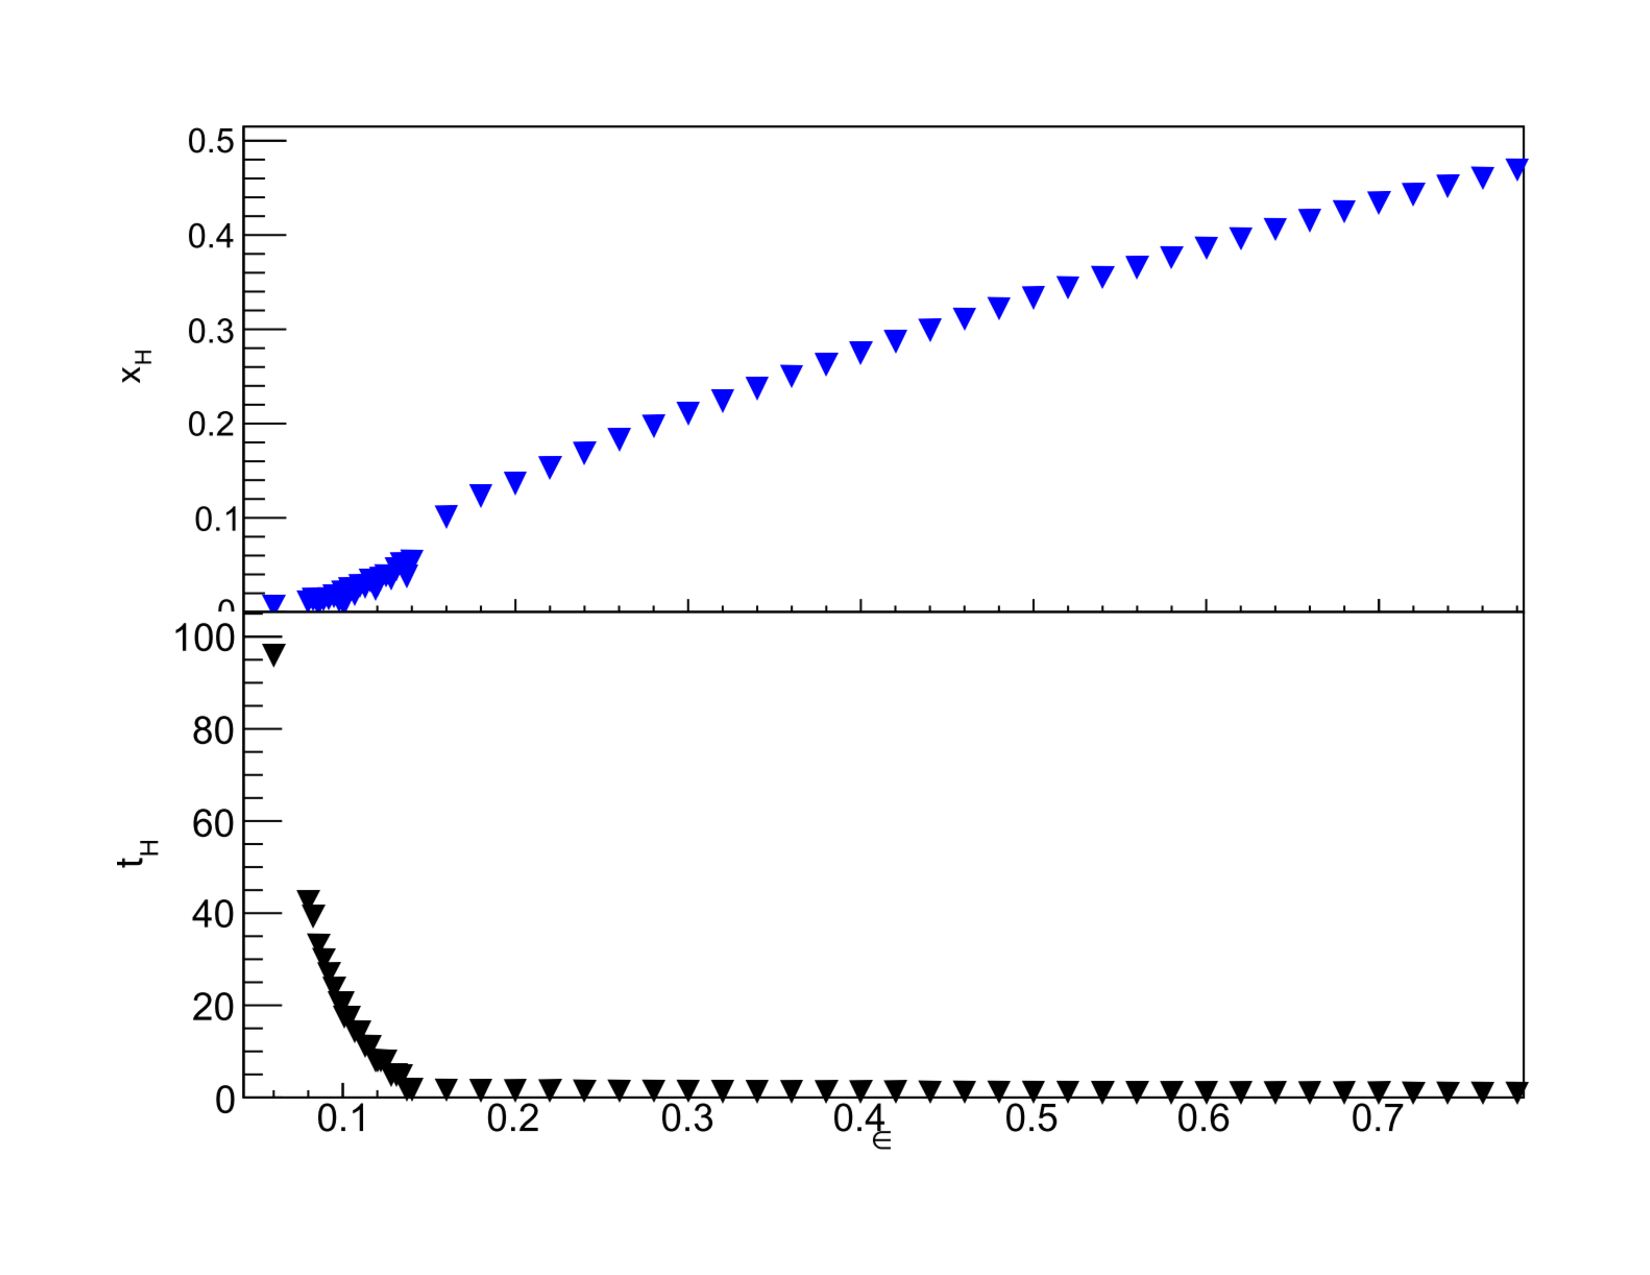
\includegraphics[width=0.65\textwidth]{/Users/bradc/Research/Thesis/PhD/Intro/figs/massive_x_vs_eps.pdf}
	\caption[Horizon size and horizon formation time for a massive scalar]{Horizon size $x_H$ and horizon formation time $t_H$ as a function of amplitude in AdS$_5$ for a massive scalar field with $\sigma = 2$ in {\rm\eqref{scalar ics}}. Instead of the periodic, discontinuous behaviour, there is some minimal value $\epsilon_{min}$ below which black holes do not form. Used with permission from {\rm\cite{1508.02709}}.}
	\label{fig: massive x vs eps}
\end{figure}

It is also worth noting as a matter of completeness that scalar field perturbations are not the only type of instabilities that have been considered. Localized, self-gravitating solutions to the Einstein-Maxwell equations in a vacuum are known as \emph{geons}, and have long lifetimes with respect to the characteristic periods of the system \cite{Wheeler:1955zz}. The excitation of a single (scalar) geon mode is stable in Anti-de Sitter space; however, any combination of two or more such modes becomes unstable \cite{1109.1825}. This complements the conjecture that the stability islands in the space of scalar field data may be anchored by linear modes. In asymptotically-AdS$_4$ spacetimes, stable geon solutions can be constructed numerically \cite{1701.09100, 1701.07804}. AdS is unstable against all vector geon modes \cite{1408.5906}.

%%%%%%%%%%%%%%%%%%%%%%%%%%%%%%%%%%%%%%%%%%%%%%%%%%%%%%%

\subsection{Driven Scalars}

We have previously limited our discussion to the normalizable scalar field solutions, as these are responsible for the weakly turbulent instabilities that lead to gravitational collapse. In general, the linearized equations of motion \eqref{collapse eigen eqn} admit two types of solutions with two different scaling behaviours near the boundary. The second set of solutions, which scale as $z^{\Delta^-}$ as $z \to 0$, are known as non-normalizable solutions and are not restricted to integer frequencies. These solutions can couple to time-dependent terms on the boundary, thereby carrying energy into the bulk, and are known as driven, or \emph{pumped}, scalar fields.

The emergence of new phases in a Conformal Field Theory as a function of driving frequency is known as Floquet dynamics \cite{1805.00031, 1802.05285}. The holographic dual to such a system is described by the driving of a massless, complex, bulk scalar field by a time-dependent boundary term. The vacuum bulk solution corresponds to a Floquet condensate on the boundary. Such solutions exhibit both stable and unstable evolution over the space of initial data, with the unstable data branching into two possible endpoints: the formation of a black hole in the bulk theory, or a horizonless, pulsating, late-time solution \cite{1612.07701, 1712.07637}. For real scalar fields subject to monotonically increasing boundary conditions, both stable and unstable data exist; however, unstable data can result in either a black hole solution, or a limiting cycle. When periodic boundary conditions are considered, dynamically stabilized big crunch singularities are possible for sufficiently high driving frequencies \cite{1206.2902}. 

Despite constructing stable and unstable numerical solutions for driven scalars, analytic solutions to the perturbative description of weakly turbulent instabilities has yet to extend beyond leading order in the backreacton with the metric \cite{1308.2132}. Capturing $\mc O(\epsilon^3)$ instabilities in these driven scalar systems is the focus of the work in chapter~\ref{ch: driven}. 


%%%%%%%%%%%%%%%%%%%%%%%%%%%%%%%%%%%%%%%%%%%%%%%%%%%%%%%
%%%%%%%%%%%%%%%%%%%%%%%%%%%%%%%%%%%%%%%%%%%%%%%%%%%%%%%

\section{Summary}
\label{sec: summary}

We have now seen how the AdS/CFT correspondence establishes a duality between strongly-coupled gauge theories and weakly-coupled gravitational theories in one extra dimension. Using this correspondence, various dynamical processes in strongly-coupled gauge theories can be explored via the collapse of scalar fields in Anti-de Sitter spacetime. Furthermore, we have seen that the end state of the theory depends on the initial profile of the scalar field, and that a large variety of both stable and unstable phenomena are possible. However, a better understanding of the islands of stability in the full theory, as well as the limits of the perturbative description, is still required. Similarly, the incorporation of time dependent boundary conditions into a perturbative theory for the weakly turbulent instabilities remains an outstanding issue. The work collected in this thesis aims to address these issues.

The following chapters each contain a manuscript that is focused on research into one of the areas described above. After a brief discussion of how each project contributes to the resolution of these issues, the contributions of the authors are laid out. The work itself is then presented. A discussion of how these works contribute to a better understanding of gravitational collapse in Anti-de Sitter space follows in chapter~\ref{ch: conclusion}.

%%%%%%%%%%%%%%%%%%%%%%%%%%%%%%%%%%%%%%%%%%%%%%%%%%%%%%%
%%%%%%%%%%%%%%%%%%%%%%%%%%%%%%%%%%%%%%%%%%%%%%%%%%%%%%%


%%%%%%%%%%%%%%%%%%%%%%%%%%%%%%%%%%%%%%%%%%%%%%%%%%%%%%%
%%%%%%%%%%%%%%%%%%%%%%%%%%%%%%%%%%%%%%%%%%%%%%%%%%%%%%%

\end{document}

%%%%%%%%%%%%%%%%%%%%%%%%%%%%%%%%%%%%%%%%%%%%%%%%%%%%%%
%%%%%%%%%%%%%%%%%%%%%%%%%%%%%%%%%%%%%%%%%%%%%%%%%%%%%%










